\documentclass[12pt]{book}
\usepackage[top=30mm, left=40mm, right=30mm, bottom=30mm]{geometry}
\usepackage[utf8]{vietnam}
\usepackage{amsthm}
\usepackage{amsmath}
\usepackage{amsfonts}
\usepackage{amssymb}
\usepackage{graphicx}
\usepackage{array}
\usepackage{makecell}
\usepackage{tabularx}
\usepackage{booktabs}
\usepackage{multicol}
\usepackage{multirow}
\usepackage{float}
\usepackage{placeins}
\usepackage{url}
\usepackage{cases}

\title{\textbf{Phân tích thiết kế hệ thống "Đăng ký lớp học"}}
\author{
  Ngô Quang Dương
}
\date{\today}

\begin{document}

\maketitle

\tableofcontents

\chapter{Mở đầu}

  \section{Đặt vấn đề}

  \section{Hệ thống hiện tại}

  \section{Hướng giải quyết}

\chapter{Thu thập và phân tích yêu cầu}
  
  \section{Bảng thuật ngữ}
    \begin{itemize}
      \item \textbf{Người dùng}: Những người có tài khoản trong hệ thống đăng ký môn học.
      \item \textbf{Sinh viên}: Những người theo học tại trường. Sinh viên theo học một khoa nào đó.
      \item \textbf{Chuyên viên}: Những người làm việc ở phòng công tác sinh viên.
      \item \textbf{Giảng viên}: Người tham gia vào việc giảng dạy. Giảng viên thuộc một khoa nào đó hoặc không. Trong một học kỳ, giảng viên có thể giảng dạy một số môn học tại một số lớp. Tuy nhiên giảng viên chỉ dạy môn học thuộc khoa của mình.
      \item \textbf{Khoa}: Đơn vị mà giảng viên làm việc, sinh viên theo học.
      \item \textbf{Môn học}: Phần kiến thức chuyên về một mảng nào đó, ví dụ như \textbf{giải tích}, \textbf{toán rời rạc}, \textbf{lập trình hướng đối tượng}, \ldots Một môn học có thể thuộc một khoa nào đó hoặc không.
      \item \textbf{Lớp môn học}: Một môn học có thể được chia ra làm nhiều lớp. Chẳng hạn với môn cơ sở dữ liệu (mã môn học là \textbf{INT2207}) có các lớp \textbf{INT2207 1}, \textbf{INT2207 2}, \textbf{INT2207 3}, \ldots
      \item \textbf{Buổi lý thuyết}: Mọi lớp học đều có duy nhất một buổi lý thuyết.
      \item \textbf{Buổi thực hành}: Một lớp học có thể có nhiều hoặc không có buổi thực hành nào.
    \end{itemize}
  
  \section{Tác nhân hệ thống}
    \begin{itemize}
      \item Quản trị hệ thống.
      \item Sinh viên.
      \item Chuyên viên.
      \item Giảng viên.
    \end{itemize}
  
  \section{Yêu cầu chức năng}
    \paragraph{Chức năng chung:}
    \begin{itemize}
      \item Đăng nhập/đăng xuất.
      \item Chỉnh sửa thông tin tài khoản.
      \item Tìm kiếm lớp học.
      \item Tìm kiếm môn học.
      \item Xem thông tin lớp học.
      \item Xem thông tin môn học.
    \end{itemize}

    \paragraph{Chức năng dành cho quản trị hệ thống:}
    \begin{itemize}
      \item Quản lý người dùng.
      \begin{itemize}
        \item Xem thông tin người dùng.
        \item Tìm kiếm người dùng.
        \item Tạo người dùng mới.
        \item Chỉnh sửa thông tin.
        \item Xóa người dùng.
      \end{itemize}
      \item Quản lý môn học:
      \begin{itemize}
        \item Tạo môn học/lớp môn học mới.
        \item Chỉnh sửa thông tin môn học/lớp môn học.
        \item Xóa môn học/lớp môn học.
      \end{itemize}
      \item Quản lý lớp học:
      \begin{itemize}
        \item Tạo lớp học mới.
        \item Đặt thời khóa biểu.
        \item Chỉnh sửa thông tin lớp học.
        \item Xóa lớp học.
      \end{itemize}
      \item Mở/đóng hệ thống:
      \begin{itemize}
        \item Cho sinh viên, chuyên viên đăng ký môn học.
        \item Cho giảng viên sắp xếp thời khóa biểu.
      \end{itemize}
    \end{itemize}

    \paragraph{Chức năng dành cho sinh viên:}
    \begin{itemize}
      \item Xem thông tin giảng viên.
      \item Tìm kiếm giảng viên.
      \item Đăng ký môn học.
      \begin{itemize}
        \item Tìm kiếm lớp học.
        \item Đăng ký lớp học mới.
        \item Bỏ lớp học đã chọn.
        \item Xem danh sách các lớp đã đăng ký.
      \end{itemize}
    \end{itemize}

    \paragraph{Chức năng dành cho chuyên viên:}
    \begin{itemize}
      \item Tìm kiếm sinh viên.
      \item Xem thông tin sinh viên.
      \item Chọn sinh viên (để thực hiện việc đăng ký môn học)
      \begin{itemize}
        \item Đăng ký môn học mới.
        \item Hủy môn học đã chọn.
        \item Xem danh sách các môn đã đăng ký.
      \end{itemize}
    \end{itemize}

    \paragraph{Chức năng dành cho giảng viên:}
    \begin{itemize}
      \item Chọn/hủy lớp giảng dạy.
      \item Xem danh sách các lớp đã nhận.
    \end{itemize}

  \section{Yêu cầu phi chức năng}
    \paragraph{
      \textnormal{
        Qua khảo sát đối với người dùng là sinh viên, hệ thống cần được đáp ứng các yêu cầu sau:
      }
    }
    \begin{itemize}
      \item Kết nối nhanh.
      \item Thời gian thực.
      \item Giao diện dễ sử dụng.
      \item Dễ tìm kiếm môn học cần đăng ký.
    \end{itemize}
  
  \section{Điều kiện ràng buộc}
    \paragraph{Đối với quản trị hệ thống:}
    \begin{itemize}
      \item Không được xóa môn học đã có lớp.
      \item Không được xóa lớp học đã có sinh viên đăng ký.
    \end{itemize}

    \paragraph{Đối với sinh viên và chuyên viên:}
    \begin{itemize}
      \item Không đăng ký quá 2 môn giáo dục thể chất.
      \item Không đăng ký môn học đã qua với điểm cao hơn $ D $.
      \item Không đăng ký nhiều hơn 1 lớp cùng một môn.
      \item Không đăng ký 2 môn học trùng thời khóa biểu.
      \item Số tín chỉ không vượt quá $ 40 $.
    \end{itemize}

    \paragraph{Đối với giảng viên:}
    \begin{itemize}
      \item Không nhận hai lớp bị trùng thời khóa biểu.
      \item Chỉ được nhận lớp thuộc môn học ở khoa mà giảng viên đó giảng dạy.
    \end{itemize}

\chapter{Đặc tả yêu cầu}

  \section{Các sơ đồ use case}

  \FloatBarrier
  \begin{figure}[ht]
    \centering
    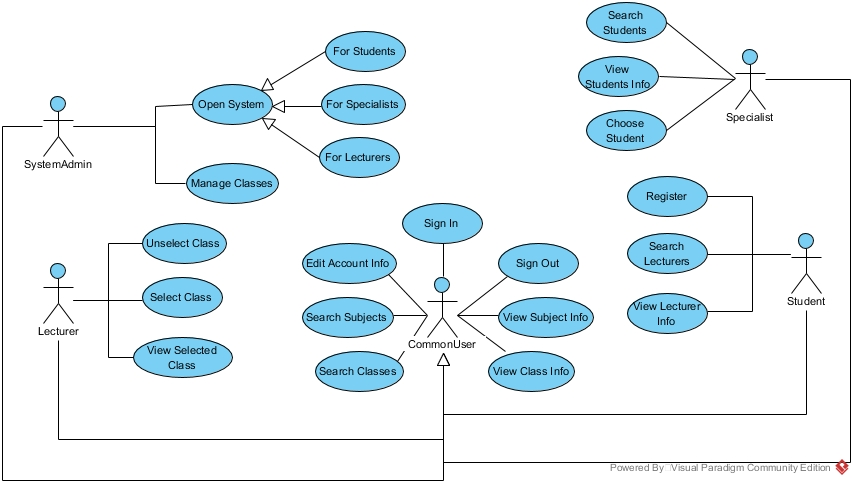
\includegraphics[scale=0.4]{../pictures/projectdiagrams/uc.jpg}
    \caption{Sơ đồ use case tổng quan}
  \end{figure}
  \FloatBarrier

  \paragraph{
    \textnormal{Do khả năng tận dụng diện tích có hạn nên một số use case được thể hiện trong các sơ đồ use case phân rã như dưới đây}
  }

  \FloatBarrier
  \begin{figure}[ht]
    \centering
    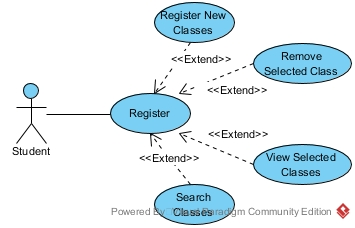
\includegraphics[scale=0.5]{../pictures/projectdiagrams/Register-uc-destructing.jpg}
    \caption{Sơ đồ phân rã cho use case đăng ký môn học}
  \end{figure}
  \FloatBarrier

  \FloatBarrier
  \begin{figure}[ht]
    \centering
    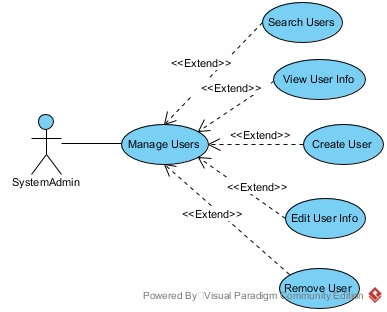
\includegraphics[scale=0.5]{../pictures/projectdiagrams/Manage-Users-uc-destructing.jpg}
    \caption{Sơ đồ phân rã cho use case quản lý người dùng}
  \end{figure}
  \FloatBarrier

  \FloatBarrier
  \begin{figure}[ht]
    \centering
    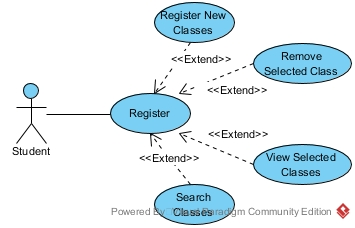
\includegraphics[scale=0.5]{../pictures/projectdiagrams/Manage-Subjects-uc-destructing.jpg}
    \caption{Sơ đồ phân rã cho use case quản lý môn học}
  \end{figure}
  \FloatBarrier

  \FloatBarrier
  \begin{figure}[ht]
    \centering
    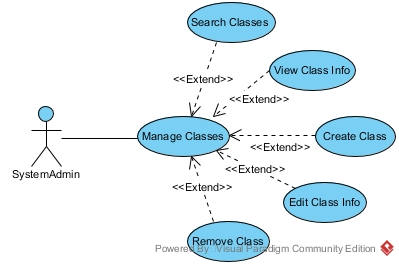
\includegraphics[scale=0.5]{../pictures/projectdiagrams/Manage-Classes-uc-destructing.jpg}
    \caption{Sơ đồ phân rã cho use case quản lý lớp học}
  \end{figure}
  \FloatBarrier

  \FloatBarrier
  \begin{figure}[ht]
    \centering
    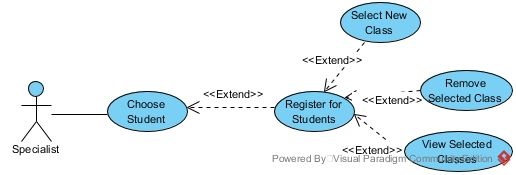
\includegraphics[scale=0.5]{../pictures/projectdiagrams/Choose-Student-uc-destructing.jpg}
    \caption{Sơ đồ phân rã cho use case chọn sinh viên}
  \end{figure}
  \FloatBarrier

  \newpage
  \section{Đặc tả use case dưới dạng bảng}

  \subsection{Use case chung}

  % Đăng nhập
  % common01
  \FloatBarrier
  \begin{table}[ht]
    \centering
    \caption{\textbf{Đăng nhập}}
    \begin{tabularx}{\textwidth}{lXX}
      \toprule
      \textbf{Tên use case:} Đăng nhập & \multicolumn{2}{l}{\textbf{ID:} common01} \\
      \hline
      \multicolumn{3}{l}{\textbf{Tác nhân chính:} Tất cả} \\
      \hline
      \textbf{Mức độ quan trọng:} cao & \multicolumn{2}{l}{\textbf{Loại use case:} hệ thống} \\
      \hline
      \multicolumn{3}{l}{\textbf{Mô tả: }Xác thực người dùng dựa vào tên đăng nhập và mật khẩu} \\
      \hline
      \multicolumn{3}{p{0.95\textwidth}}{
        \textbf{Điều kiện khởi phát: }Người dùng truy cập vào hệ thống mà chưa được xác thực thành công.
      } \\
      \hline
      \multicolumn{3}{l}{
        \makecell[l]{
          \textbf{Quan hệ với các use case khác:}\\
          -- Để có thể thực hiện các use case khác, cần đăng nhập trước.
        }
      }\\
      \hline
      \multicolumn{3}{l}{\textbf{Luồng hoạt động chính:}} \\
      \hline
      TT $\qquad$ Thực hiện bởi & \multicolumn{2}{l}{Hành động} \\
      \hline
      $\quad 1\qquad\quad$ Người dùng & \multicolumn{2}{l}{Nhập thông tin đăng nhập} \\
      \hline
      $\quad 2\qquad\quad$ Người dùng & \multicolumn{2}{l}{Gửi yêu cầu đăng nhập} \\
      \hline
      $\quad 3\qquad\quad$ Hệ thống & \multicolumn{2}{l}{Kiểm tra thông tin đăng nhập} \\
      \hline
      $\quad 4\qquad\quad$ Hệ thống & \multicolumn{2}{l}{Điều hướng đến trang chính}\\
      \hline
      \multicolumn{3}{l}{\textbf{Luồng hoạt động con:}} \\
      \hline
      $\ 3.1\qquad\quad$ Hệ thống & \multicolumn{2}{l}{Thông báo thông tin đăng nhập sai} \\
      \bottomrule
    \end{tabularx}
  \end{table}
  \FloatBarrier

  % Đăng xuất
  % common02
  \FloatBarrier
  \begin{table}[ht]
    \centering
    \caption{Đăng xuất}
    \begin{tabularx}{\textwidth}{lXX}
      \toprule
      \textbf{Tên use case:} Đăng xuất & \multicolumn{2}{l}{\textbf{ID:} common02} \\
      \hline
      \multicolumn{3}{l}{\textbf{Tác nhân chính:} Tất cả} \\
      \hline
      \textbf{Mức độ quan trọng:} trung bình & \multicolumn{2}{l}{\textbf{Loại use case:} hệ thống} \\
      \hline
      \multicolumn{3}{l}{\textbf{Mô tả: }Rời khỏi hệ thống} \\
      \hline
      \multicolumn{3}{p{0.95\textwidth}}{
        \textbf{Điều kiện khởi phát: }Người dùng yêu cầu đăng xuất
      } \\
      \hline
      \multicolumn{3}{l}{
        \makecell[l]{
          \textbf{Quan hệ với các use case khác:}\\
          -- Phụ thuộc vào use case đăng nhập.
        }
      }\\
      \hline
      \multicolumn{3}{l}{\textbf{Luồng hoạt động chính:}} \\
      \hline
      TT $\qquad$ Thực hiện bởi & \multicolumn{2}{l}{Hành động} \\
      \hline
      $\quad 1\qquad\quad$ Người dùng & \multicolumn{2}{l}{Chọn đăng xuất} \\
      \hline
      $\quad 2\qquad\quad$ Hệ thống & \multicolumn{2}{l}{Xóa session/cookie} \\
      \bottomrule
    \end{tabularx}
  \end{table}
  \FloatBarrier

  % Sửa thông tin tài khoản
  % common03
  \FloatBarrier
  \begin{table}[ht]
    \centering
    \caption{Sửa thông tin tài khoản}
    \begin{tabularx}{\textwidth}{lXX}
      \toprule
      \multicolumn{2}{l}{\textbf{Tên use case: }Sửa thông tin tài khoản} & \textbf{ID: }common03 \\
      \hline
      \multicolumn{3}{l}{\textbf{Tác nhân chính: }Tất cả} \\
      \hline
      \textbf{Mức độ quan trọng: }trung bình & \multicolumn{2}{l}{\textbf{Loại use case: }hệ thống} \\
      \hline
      \multicolumn{3}{l}{\textbf{Mô tả: }Sửa các thông tin như \textit{thông tin cá nhân}, \textit{email}, \textit{mật khẩu}, \ldots} \\
      \hline
      \multicolumn{3}{l}{
        \textbf{Điều kiện khởi phát: }Người dùng truy cập trang chỉnh sửa thông tin tài khoản
      } \\
      \hline
      \multicolumn{3}{l}{
        \makecell[l]{
          \textbf{Quan hệ với các use case khác:} \\
          -- Phụ thuộc vào use case đăng nhập.
        }
      } \\
      \hline
      \multicolumn{3}{l}{\textbf{Luồng hoạt động chính:}} \\
      \hline
      TT $\qquad$ Thực hiện bởi & \multicolumn{2}{l}{Hành động} \\
      \hline
      $\quad 1\qquad\quad$ Người dùng & \multicolumn{2}{l}{Nhập lại những thông tin cần chỉnh sửa} \\
      \hline
      $\quad 2\qquad\quad$ Người dùng & \multicolumn{2}{l}{Gửi yêu cầu sửa} \\
      \hline
      $\quad 3\qquad\quad$ Hệ thống & \multicolumn{2}{l}{Kiểm tra tính hợp lý của thông tin mới} \\
      \hline
      $\quad 4\qquad\quad$ Hệ thống & \multicolumn{2}{l}{Cập nhật thông tin mới} \\
      \bottomrule
    \end{tabularx}
  \end{table}
  \FloatBarrier

  % Tìm kiếm môn học
  % common04
  \FloatBarrier
  \begin{table}[ht]
    \centering
    \caption{Tìm kiếm môn học}
    \begin{tabularx}{\textwidth}{lXX}
      \toprule
      \multicolumn{2}{l}{
        \textbf{Tên use case: }Tìm kiếm môn học
      } & \textbf{ID: }common04 \\
      \hline
      \multicolumn{3}{l}{
        \textbf{Tác nhân chính: }quản trị hệ thống
      } \\
      \hline
      \textbf{Mức độ quan trọng: }trung bình & \multicolumn{2}{l}{\textbf{Loại use case: }nghiệp vụ} \\
      \hline
      \multicolumn{3}{l}{
        \makecell[l]{
          \textbf{Mô tả: }Tìm kiếm môn học dựa trên các thuộc tính như \textit{từ khóa}, \textit{khoa}, \ldots}
      }\\
      \hline
      \multicolumn{3}{l}{
        \textbf{Điều kiện khởi phát: }Quản trị viên sử dụng form tìm kiếm môn học
      }\\
      \hline
      \multicolumn{3}{l}{
        \makecell[l]{
          \textbf{Quan hệ với các use case khác:}\\
          -- Phụ thuộc vào use case đăng nhập.
        }
      } \\
      \hline
      \multicolumn{3}{l}{\textbf{Luồng hoạt động chính:}}\\
      \hline
      TT $\qquad$ Thực hiện bởi & \multicolumn{2}{l}{Hành động} \\
      \hline
      $\quad 1\qquad\quad$ Quản trị hệ thống & \multicolumn{2}{l}{
        \makecell[l]{
          Nhập thông tin tìm kiếm
        }
      } \\
      \hline
      $\quad 2\qquad\quad$ Quản trị hệ thống & \multicolumn{2}{l}{Gửi yêu cầu tìm kiếm} \\
      \hline
      $\quad 3\qquad\quad$ Hệ thống & \multicolumn{2}{l}{Tìm kiếm dựa trên thông tin yêu cầu} \\
      \hline
      $\quad 4\qquad\quad$ Hệ thống & \multicolumn{2}{l}{Hiển thị kết quả tìm kiếm} \\
      \bottomrule
    \end{tabularx}
  \end{table}
  \FloatBarrier

  % Xem thông tin môn học
  % common05
  \FloatBarrier
  \begin{table}[ht]
    \centering
    \caption{Xem thông tin môn học}
    \begin{tabularx}{\textwidth}{lXX}
      \toprule
      \multicolumn{2}{l}{\textbf{Tên use case: }Xem thông tin môn học} & \textbf{ID: }common05 \\
      \hline
      \multicolumn{3}{l}{\textbf{Tác nhân chính: }quản trị hệ thống} \\
      \hline
      \textbf{Mức độ quan trọng: }thấp & \multicolumn{2}{l}{\textbf{Loại use case: }nghiệp vụ} \\
      \hline
      \multicolumn{3}{l}{
        \makecell[l]{
          \textbf{Mô tả: }Xem tất cả thông tin của môn học được chọn
        }
      } \\
      \hline
      \multicolumn{3}{l}{\textbf{Điều kiện khởi phát: }Quản trị hệ thống chọn một môn học cụ thể} \\
      \hline
      \multicolumn{3}{l}{
        \makecell[l]{
          \textbf{Quan hệ với các use case khác:} \\
          -- Phụ thuộc vào use case đăng nhập
        }
      } \\
      \hline
      \multicolumn{3}{l}{\textbf{Luồng hoạt động chính:}} \\
      \hline
      TT $\qquad\quad$ Thực hiện bởi & \multicolumn{2}{l}{Hành động} \\
      \hline
      $\quad 1\qquad\quad$ Hệ thống & \multicolumn{2}{l}{Hiển thị tất cả thông tin về môn học} \\
      \bottomrule
    \end{tabularx}
  \end{table}
  \FloatBarrier

  % Tìm kiếm lớp học
  % common06
  \FloatBarrier
  \begin{table}[ht]
    \centering
    \caption{Tìm kiếm lớp học}
    \begin{tabularx}{\textwidth}{lXX}
      \toprule
      \multicolumn{2}{l}{
        \textbf{Tên use case: }Tìm kiếm lớp học
      } & \textbf{ID: }common06 \\
      \hline
      \multicolumn{3}{l}{
        \textbf{Tác nhân chính: }quản trị hệ thống
      } \\
      \hline
      \textbf{Mức độ quan trọng: }trung bình & \multicolumn{2}{l}{\textbf{Loại use case: }nghiệp vụ} \\
      \hline
      \multicolumn{3}{l}{
        \makecell[l]{
          \textbf{Mô tả: }Tìm kiếm lớp học dựa trên các thuộc tính như \textit{từ khóa}, \textit{môn học}, \ldots}
      }\\
      \hline
      \multicolumn{3}{l}{
        \textbf{Điều kiện khởi phát: }Quản trị viên sử dụng form tìm kiếm lớp học
      }\\
      \hline
      \multicolumn{3}{l}{
        \makecell[l]{
          \textbf{Quan hệ với các use case khác:}\\
          -- Phụ thuộc vào use case đăng nhập.
        }
      } \\
      \hline
      \multicolumn{3}{l}{\textbf{Luồng hoạt động chính:}}\\
      \hline
      TT $\qquad$ Thực hiện bởi & \multicolumn{2}{l}{Hành động} \\
      \hline
      $\quad 1\qquad\quad$ Quản trị hệ thống & \multicolumn{2}{l}{
        \makecell[l]{
          Nhập thông tin tìm kiếm
        }
      } \\
      \hline
      $\quad 2\qquad\quad$ Quản trị hệ thống & \multicolumn{2}{l}{Gửi yêu cầu tìm kiếm} \\
      \hline
      $\quad 3\qquad\quad$ Hệ thống & \multicolumn{2}{l}{Tìm kiếm lớp học dựa trên thông tin yêu cầu} \\
      \hline
      $\quad 4\qquad\quad$ Hệ thống & \multicolumn{2}{l}{Hiển thị kết quả tìm kiếm} \\
      \bottomrule
    \end{tabularx}
  \end{table}
  \FloatBarrier

  % Xem thông tin lớp học
  % common07
  \FloatBarrier
  \begin{table}[ht]
    \centering
    \caption{Xem thông tin lớp học}
    \begin{tabularx}{\textwidth}{lXX}
      \toprule
      \multicolumn{2}{l}{\textbf{Tên use case: }Xem thông tin lớp học} & \textbf{ID: }common07 \\
      \hline
      \multicolumn{3}{l}{\textbf{Tác nhân chính: }quản trị hệ thống} \\
      \hline
      \textbf{Mức độ quan trọng: }thấp & \multicolumn{2}{l}{\textbf{Loại use case: }nghiệp vụ} \\
      \hline
      \multicolumn{3}{l}{
        \makecell[l]{
          \textbf{Mô tả: }Xem tất cả thông tin của môn học được chọn
        }
      } \\
      \hline
      \multicolumn{3}{l}{\textbf{Điều kiện khởi phát: }Quản trị hệ thống chọn một môn học cụ thể} \\
      \hline
      \multicolumn{3}{l}{
        \makecell[l]{
          \textbf{Quan hệ với các use case khác:} \\
          -- Phụ thuộc vào use case đăng nhập
        }
      } \\
      \hline
      \multicolumn{3}{l}{\textbf{Luồng hoạt động chính:}} \\
      \hline
      TT $\qquad\quad$ Thực hiện bởi & \multicolumn{2}{l}{Hành động} \\
      \hline
      $\quad 1\qquad\quad$ Hệ thống & \multicolumn{2}{l}{Hiển thị tất cả thông tin về môn học} \\
      \bottomrule
    \end{tabularx}
  \end{table}
  \FloatBarrier
  
  \subsection{Dành cho quản trị hệ thống}
  % Đóng/mở hệ thống cho giảng viên
  % sa01
  \FloatBarrier
  \begin{table}[ht]
    \centering
    \caption{Đóng/mở hệ thống cho giảng viên}
    \begin{tabularx}{\textwidth}{lXX}
      \toprule
      \multicolumn{2}{l}{\textbf{Tên use case: }Đóng/mở hệ thống cho giảng viên} & \textbf{ID: }sa01 \\
      \hline
      \multicolumn{3}{l}{\textbf{Tác nhân chính: }quản trị hệ thống} \\
      \hline
      \textbf{Mức độ quan trọng: }cao & \multicolumn{2}{l}{\textbf{Loại use case: }hệ thống} \\
      \hline
      \multicolumn{3}{l}{\textbf{Mô tả: }Cho phép giảng viên chọn lớp} \\
      \hline
      \multicolumn{3}{l}{\textbf{Điều kiện khởi phát: }Quản trị viên chọn chức năng} \\
      \hline
      \multicolumn{3}{l}{
        \makecell[l]{
          \textbf{Quan hệ với các use case khác:}\\
          -- Phụ thuộc vào use case đăng nhập.
        }
      } \\
      \hline
      \multicolumn{3}{l}{\textbf{Luồng hoạt động chính:}} \\
      \hline
      TT $\qquad$ Thực hiện bởi & Hành động \\
      \hline
      $\quad 1\qquad\quad$ Quản trị hệ thống & \multicolumn{2}{l}{
        \makecell[l]{
          Chọn chức năng đóng hoặc mở hệ thống đối với\\ giảng viên}
      } \\
      \hline
      $\quad 2\qquad\quad$ Hệ thống & \multicolumn{2}{l}{Đóng hệ thống đối với các tác nhân khác} \\
      \hline
      \multicolumn{3}{l}{\textbf{Luồng hoạt động con:}} \\
      \hline
      $\ 1.1\qquad\quad$ Hệ thống & \multicolumn{2}{l}{Đóng hệ thống đối với giảng viên} \\
      \bottomrule
    \end{tabularx}
  \end{table}
  \FloatBarrier

  % Đóng/mở hệ thống cho chuyên viên
  % sa02
  \FloatBarrier
  \begin{table}[ht]
    \centering
    \caption{Đóng/mở hệ thống cho chuyên viên}
    \begin{tabularx}{\textwidth}{lXX}
      \toprule
      \multicolumn{2}{l}{
        \textbf{Tên use case: }Đóng/mở hệ thống cho chuyên viên
      } & \textbf{ID: }sa02 \\
      \hline
      \multicolumn{3}{l}{\textbf{Tác nhân chính: }quản trị hệ thống} \\
      \hline
      \textbf{Mức độ quan trọng: }cao & \multicolumn{2}{l}{\textbf{Loại use case: }hệ thống} \\
      \hline
      \multicolumn{3}{l}{
        \makecell[l]{
          \textbf{Mô tả: }Cho phép chuyên viên thực hiện đăng ký lớp học/chỉnh sửa đăng ký giúp\\ sinh viên
        }
      }\\
      \hline
      \multicolumn{3}{l}{
        \makecell[l]{
          \textbf{Điều kiện khởi phát: }Quản trị viên chọn chức năng}
        } \\
      \hline
      \multicolumn{3}{l}{
        \makecell[l]{
          \textbf{Quan hệ với các use case khác:}\\
          -- Phụ thuộc vào use case đăng nhập
        }
      }\\
      \hline
      \multicolumn{3}{l}{\textbf{Luồng hoạt động chính:}} \\
      \hline
      TT $\qquad$ Thực hiện bởi & \multicolumn{2}{l}{Hành động} \\
      \hline
      $\quad 1\qquad\quad$ Quản trị hệ thống & \multicolumn{2}{l}{
        \makecell[l]{Chọn chức năng đóng hoặc mở hệ thống đối với\\ chuyên viên}} \\
      \hline
      $\quad 2\qquad\quad$ Hệ thống & \multicolumn{2}{l}{Đóng hệ thống đối với giảng viên} \\
      \hline
      $\quad 3\qquad\quad$ Hệ thống & \multicolumn{2}{l}{Mở hệ thống đối với chuyên viên} \\
      \hline
      \multicolumn{3}{l}{\textbf{Luồng hoạt động con:}} \\
      \hline
      $\ 1.1\qquad\quad$ Hệ thống & \multicolumn{2}{l}{Đóng hệ thống đối với chuyên viên} \\
      \bottomrule
    \end{tabularx}
  \end{table}
  \FloatBarrier

  % Đóng/mở hệ thống cho sinh viên
  % sa03
  \FloatBarrier
  \begin{table}[ht]
    \centering
    \caption{Đóng/mở hệ thống cho sinh viên}
    \begin{tabularx}{\textwidth}{lXX}
      \toprule
      \multicolumn{2}{l}{
        \textbf{Tên use case: }Đóng/mở hệ thống cho sinh viên
      } & \textbf{ID: }sa03 \\
      \hline
      \multicolumn{3}{l}{
        \textbf{Tác nhân chính: } quản trị hệ thống
      } \\
      \hline
      \textbf{Mức độ quan trọng: }cao & \multicolumn{2}{l}{\textbf{Loại use case: }hệ thống} \\
      \hline
      \multicolumn{3}{l}{
        \makecell[l]{
          \textbf{Mô tả: }Cho phép sinh viên đăng ký lớp học
        }
      } \\
      \hline
      \multicolumn{3}{l}{
        \textbf{Điều kiện khởi phát: }Quản trị viên chọn chức năng
      } \\
      \hline
      \multicolumn{3}{l}{
        \makecell[l]{
          \textbf{Quan hệ với các use case khác:}\\
          -- Phụ thuộc vào use case đăng nhập.
        }
      }\\
      \hline
      \multicolumn{3}{l}{\textbf{Luồng hoạt động chính:}}\\
      \hline
      TT $\quad\qquad$ Thực hiện bởi & Hành động \\
      \hline
      $\quad 1\qquad\quad$ Quản trị hệ thống & \multicolumn{2}{l}{
        \makecell[l]{
          Chọn chức năng đóng hoặc mở hệ thống đối với\\
          sinh viên
        }
      } \\
      \hline
      $\quad 2\qquad\quad$ Hệ thống & \multicolumn{2}{l}{Đóng hệ thống đối với giảng viên} \\
      \hline
      $\quad 3\qquad\quad$ Hệ thống & \multicolumn{2}{l}{Mở hệ thống đối với sinh viên} \\
      \hline
      \multicolumn{3}{l}{\textbf{Luồng hoạt động con:}} \\
      \hline
      $\ 1.1\qquad\quad$ Hệ thống & \multicolumn{2}{l}{Đóng hệ thống đối với sinh viên} \\
      \bottomrule
    \end{tabularx}
  \end{table}
  \FloatBarrier

  %% Quản lý người dùng

  % Tìm kiếm người dùng
  % sa04
  \FloatBarrier
  \begin{table}[ht]
    \centering
    \caption{Tìm kiếm người dùng}
    \begin{tabularx}{\textwidth}{lXX}
      \toprule
      \multicolumn{2}{l}{
        \textbf{Tên use case: }Tìm kiếm người dùng
      } & \textbf{ID: }sa04 \\
      \hline
      \multicolumn{3}{l}{
        \textbf{Tác nhân chính: }quản trị hệ thống
      } \\
      \hline
      \textbf{Mức độ quan trọng: }trung bình & \multicolumn{2}{l}{\textbf{Loại use case: }nghiệp vụ} \\
      \hline
      \multicolumn{3}{l}{
        \makecell[l]{
          \textbf{Mô tả: }Tìm kiếm người dùng dựa trên các thuộc tính như \textit{từ khóa}, \textit{chức vụ}, \ldots}
      }\\
      \hline
      \multicolumn{3}{l}{
        \textbf{Điều kiện khởi phát: }Quản trị viên sử dụng form tìm kiếm người dùng
      }\\
      \hline
      \multicolumn{3}{l}{
        \makecell[l]{
          \textbf{Quan hệ với các use case khác:}\\
          -- Phụ thuộc vào use case đăng nhập.
        }
      } \\
      \hline
      \multicolumn{3}{l}{\textbf{Luồng hoạt động chính:}}\\
      \hline
      TT $\qquad$ Thực hiện bởi & \multicolumn{2}{l}{Hành động} \\
      \hline
      $\quad 1\qquad\quad$ Quản trị hệ thống & \multicolumn{2}{l}{
        \makecell[l]{
          Nhập thông tin tìm kiếm
        }
      } \\
      \hline
      $\quad 2\qquad\quad$ Quản trị hệ thống & \multicolumn{2}{l}{Gửi yêu cầu tìm kiếm} \\
      \hline
      $\quad 3\qquad\quad$ Hệ thống & \multicolumn{2}{l}{Tìm kiếm dựa trên thông tin yêu cầu} \\
      \hline
      $\quad 4\qquad\quad$ Hệ thống & \multicolumn{2}{l}{Hiển thị kết quả tìm kiếm} \\
      \bottomrule
    \end{tabularx}
  \end{table}
  \FloatBarrier

  % Xem thông tin người dùng
  % sa05
  \FloatBarrier
  \begin{table}[ht]
    \centering
    \caption{Xem thông tin người dùng}
    \begin{tabularx}{\textwidth}{lXX}
      \toprule
      \multicolumn{2}{l}{\textbf{Tên use case: }Xem thông tin người dùng} & \textbf{ID: }sa05 \\
      \hline
      \multicolumn{3}{l}{\textbf{Tác nhân chính: }quản trị hệ thống} \\
      \hline
      \textbf{Mức độ quan trọng: }thấp & \multicolumn{2}{l}{\textbf{Loại use case: }nghiệp vụ} \\
      \hline
      \multicolumn{3}{l}{
        \makecell[l]{
          \textbf{Mô tả: }xem tất cả thông tin của người dùng hệ thống (trừ mật khẩu, mật khẩu\\ được băm)
        }
      } \\
      \hline
      \multicolumn{3}{l}{\textbf{Điều kiện khởi phát: }Quản trị hệ thống chọn một người dùng cụ thể} \\
      \hline
      \multicolumn{3}{l}{
        \makecell[l]{
          \textbf{Quan hệ với các use case khác:} \\
          -- Phụ thuộc vào use case đăng nhập
        }
      } \\
      \hline
      \multicolumn{3}{l}{\textbf{Luồng hoạt động chính:}} \\
      \hline
      TT $\qquad\quad$ Thực hiện bởi & \multicolumn{2}{l}{Hành động} \\
      \hline
      $\quad 1\qquad\quad$ Hệ thống & \multicolumn{2}{l}{Hiển thị tất cả thông tin về người dùng}\\
      \bottomrule
    \end{tabularx}
  \end{table}
  \FloatBarrier

  % Tạo người dùng mới
  % sa06
  \FloatBarrier
  \begin{table}[ht]
    \centering
    \caption{Tạo người dùng mới}
    \begin{tabularx}{\textwidth}{lXX}
      \toprule
      \multicolumn{2}{l}{\textbf{Tên use case: }Xem thông tin người dùng} & \textbf{ID: }sa06 \\
      \hline
      \multicolumn{3}{l}{\textbf{Tác nhân chính: }quản trị hệ thống} \\
      \hline
      \textbf{Mức độ quan trọng: }trung bình & \multicolumn{2}{l}{\textbf{Loại use case: }nghiệp vụ} \\
      \hline
      \multicolumn{3}{l}{
        \makecell[l]{
          \textbf{Mô tả: }Tạo một tài khoản mới
        }
      } \\
      \hline
      \multicolumn{3}{l}{\textbf{Điều kiện khởi phát: }Quản trị hệ thống truy cập trang tạo người dùng mới} \\
      \hline
      \multicolumn{3}{l}{
        \makecell[l]{
          \textbf{Quan hệ với các use case khác:} \\
          -- Phụ thuộc vào use case đăng nhập
        }
      } \\
      \hline
      \multicolumn{3}{l}{\textbf{Luồng hoạt động chính:}} \\
      \hline
      TT $\qquad\quad$ Thực hiện bởi & \multicolumn{2}{l}{Hành động} \\
      \hline
      $\quad 1\qquad\quad$ Quản trị hệ thống & \multicolumn{2}{l}{
        \makecell[l]{
          Nhập thông tin cho tài khoản mới, gồm: \\
          -- Mã người dùng. \\
          -- Chức vụ trong hệ thống (giảng viên,\\chuyên viên, sinh viên) \\
          -- Họ tên. \\
          -- Giới tính. \\
          -- Năm sinh. \\
          -- \ldots
        }
      } \\
      \hline
      $\quad 2\qquad\quad$ Quản trị hệ thống & \multicolumn{2}{l}{Gửi yêu cầu tạo tài khoản} \\
      \hline
      $\quad 3\qquad\quad$ Hệ thống & \multicolumn{2}{l}{Kiểm tra trùng lặp} \\
      \hline
      $\quad 4\qquad\quad$ Hệ thống & \multicolumn{2}{l}{Kiểm tra tính hợp lệ} \\
      \hline
      $\quad 5\qquad\quad$ Hệ thống & \multicolumn{2}{l}{Tạo tài khoản mới} \\
      \hline
      $\quad 6\qquad\quad$ Hệ thống & \multicolumn{2}{l}{Thông báo tạo tài khoản thành công} \\
      \hline
      \multicolumn{3}{l}{\textbf{Luồng hoạt động con:}} \\
      \hline
      $\ 3.1\qquad\quad$ Hệ thống & \multicolumn{2}{l}{Thông báo thông tin bị trùng lặp} \\
      \hline
      $\ 4.1\qquad\quad$ Hệ thống & \multicolumn{2}{l}{Thông báo thông tin không hợp lệ} \\
      \bottomrule
    \end{tabularx}
  \end{table}
  \FloatBarrier

  % Chỉnh sửa thông tin người dùng
  % sa07
  \FloatBarrier
  \begin{table}[ht]
    \centering
    \caption{Sửa thông tin người dùng}
    \begin{tabularx}{\textwidth}{lXX}
      \toprule
      \multicolumn{2}{l}{\textbf{Tên use case: }Sửa thông tin người dùng} & \textbf{ID: }sa07 \\
      \hline
      \multicolumn{3}{l}{\textbf{Tác nhân chính: }Quản trị hệ thống} \\
      \hline
      \textbf{Mức độ quan trọng: }trung bình & \multicolumn{2}{l}{\textbf{Loại use case: }nghiệp vụ} \\
      \hline
      \multicolumn{3}{l}{
        \makecell[l]{
          \textbf{Mô tả: }Sửa một số thông tin của người dùng
        }
      } \\
      \hline
      \multicolumn{3}{l}{\textbf{Điều kiện khởi phát: }Quản trị hệ thống chọn một người dùng cụ thể} \\
      \hline
      \multicolumn{3}{l}{
        \makecell[l]{
          \textbf{Quan hệ với các use case khác:} \\
          -- Phụ thuộc vào use case đăng nhập
        }
      } \\
      \hline
      \multicolumn{3}{l}{\textbf{Luồng hoạt động chính:}} \\
      \hline
      TT $\qquad\quad$ Thực hiện bởi & \multicolumn{2}{l}{Hành động} \\
      \hline
      $\quad 1\qquad\quad$ Quản trị hệ thống & \multicolumn{2}{l}{Chọn chức năng sửa} \\
      \hline
      $\quad 2\qquad\quad$ Quản trị hệ thống & \multicolumn{2}{l}{Nhập lại những thông tin cần sửa} \\
      \hline
      $\quad 3\qquad\quad$ Quản trị hệ thống & \multicolumn{2}{l}{Gửi yêu cầu sửa} \\
      \hline
      $\quad 4\qquad\quad$ Hệ thống & \multicolumn{2}{l}{Kiểm tra trùng lặp} \\
      \hline
      $\quad 5\qquad\quad$ Hệ thống & \multicolumn{2}{l}{Kiểm tra tính hợp lệ} \\
      \hline
      $\quad 6\qquad\quad$ Hệ thống & \multicolumn{2}{l}{Cập nhật thông tin mới} \\
      \hline
      \multicolumn{3}{l}{\textbf{Luồng hoạt động con:}} \\
      \hline
      $\ 4.1\qquad\quad$ Hệ thống & \multicolumn{2}{l}{Thông báo trùng lặp} \\
      \hline
      $\ 5.1\qquad\quad$ Hệ thống & \multicolumn{2}{l}{Thông báo thông tin không hợp lệ} \\
      \bottomrule
    \end{tabularx}
  \end{table}
  \FloatBarrier

  % Xóa người dùng
  % sa08
  \FloatBarrier
  \begin{table}[ht]
    \centering
    \caption{Xoá người dùng}
    \begin{tabularx}{\textwidth}{lXX}
      \toprule
      \multicolumn{2}{l}{\textbf{Tên use case: }Xóa người dùng} & \textbf{ID: }sa08 \\
      \hline
      \multicolumn{3}{l}{\textbf{Tác nhân chính: }quản trị hệ thống} \\
      \hline
      \textbf{Mức độ quan trọng: }thấp & \multicolumn{2}{l}{\textbf{Loại use case: }nghiệp vụ} \\
      \hline
      \multicolumn{3}{l}{
        \makecell[l]{
          \textbf{Mô tả: }Xóa tất cả thông tin, những gì liên quan đến một người dùng cụ thể
        }
      } \\
      \hline
      \multicolumn{3}{l}{\textbf{Điều kiện khởi phát: }Quản trị hệ thống chọn một người dùng cụ thể} \\
      \hline
      \multicolumn{3}{l}{
        \makecell[l]{
          \textbf{Quan hệ với các use case khác:} \\
          -- Phụ thuộc vào use case đăng nhập
        }
      } \\
      \hline
      \multicolumn{3}{l}{\textbf{Luồng hoạt động chính:}} \\
      \hline
      TT $\qquad\quad$ Thực hiện bởi & \multicolumn{2}{l}{Hành động} \\
      \hline
      $\quad 1\qquad\quad$ Quản trị hệ thống & \multicolumn{2}{l}{Gửi yêu cầu xóa một tài khoản} \\
      \hline
      $\quad 2\qquad\quad$ Hệ thống & \multicolumn{2}{l}{\makecell[l]{
        Xóa tài khoản và các thông tin liên quan
      }} \\
      \hline
      $\quad 3\qquad\quad$ Hệ thống & \multicolumn{2}{l}{Thông báo xóa thành công} \\
      \bottomrule
    \end{tabularx}
  \end{table}
  \FloatBarrier

  %% Quản lý môn học

  % Tạo môn học mới
  % sa09
  \FloatBarrier
  \begin{table}[ht]
    \centering
    \caption{Tạo môn học mới}
    \begin{tabularx}{\textwidth}{lXX}
      \toprule
      \multicolumn{2}{l}{\textbf{Tên use case: }Tạo môn học mới} & \textbf{ID: }sa09 \\
      \hline
      \multicolumn{3}{l}{\textbf{Tác nhân chính: }quản trị hệ thống} \\
      \hline
      \textbf{Mức độ quan trọng: }trung bình & \multicolumn{2}{l}{\textbf{Loại use case: }nghiệp vụ} \\
      \hline
      \multicolumn{3}{l}{
        \makecell[l]{
          \textbf{Mô tả: }Tạo một môn học mới
        }
      } \\
      \hline
      \multicolumn{3}{l}{\textbf{Điều kiện khởi phát: }Quản trị hệ thống truy cập trang tạo môn học mới} \\
      \hline
      \multicolumn{3}{l}{
        \makecell[l]{
          \textbf{Quan hệ với các use case khác:} \\
          -- Phụ thuộc vào use case đăng nhập
        }
      } \\
      \hline
      \multicolumn{3}{l}{\textbf{Luồng hoạt động chính:}} \\
      \hline
      TT $\qquad\quad$ Thực hiện bởi & \multicolumn{2}{l}{Hành động} \\
      \hline
      $\quad 1\qquad\quad$ Quản trị hệ thống & \multicolumn{2}{l}{Nhập thông tin cho môn học mới} \\
      \hline
      $\quad 2\qquad\quad$ Quản trị hệ thống & \multicolumn{2}{l}{Gửi yêu cầu tạo môn học} \\
      \hline
      $\quad 3\qquad\quad$ Hệ thống & \multicolumn{2}{l}{Kiểm tra trùng lặp} \\
      \hline
      $\quad 4\qquad\quad$ Hệ thống & \multicolumn{2}{l}{Kiểm tra tính hợp lệ} \\
      \hline
      $\quad 5\qquad\quad$ Hệ thống & \multicolumn{2}{l}{Tạo môn học mới} \\
      \hline
      $\quad 6\qquad\quad$ Hệ thống & \multicolumn{2}{l}{Thông báo tạo môn học thành công} \\
      \hline
      \multicolumn{3}{l}{\textbf{Luồng hoạt động con:}} \\
      \hline
      $\ 3.1\qquad\quad$ Hệ thống & \multicolumn{2}{l}{Thông báo thông tin bị trùng lặp} \\
      \hline
      $\ 4.1\qquad\quad$ Hệ thống & \multicolumn{2}{l}{Thông báo thông tin không hợp lệ} \\
      \bottomrule
    \end{tabularx}
  \end{table}
  \FloatBarrier

  % Chỉnh sửa thông tin môn học
  % sa10
  \FloatBarrier
  \begin{table}[ht]
    \centering
    \caption{Sửa thông tin môn học}
    \begin{tabularx}{\textwidth}{lXX}
      \toprule
      \multicolumn{2}{l}{\textbf{Tên use case: }Sửa thông tin môn học} & \textbf{ID: }sa10 \\
      \hline
      \multicolumn{3}{l}{\textbf{Tác nhân chính: }Quản trị hệ thống} \\
      \hline
      \textbf{Mức độ quan trọng: }trung bình & \multicolumn{2}{l}{\textbf{Loại use case: }nghiệp vụ} \\
      \hline
      \multicolumn{3}{l}{
        \makecell[l]{
          \textbf{Mô tả: }Sửa một số thông tin của môn học được chọn
        }
      } \\
      \hline
      \multicolumn{3}{l}{\textbf{Điều kiện khởi phát: }Quản trị hệ thống chọn một môn học cụ thể} \\
      \hline
      \multicolumn{3}{l}{
        \makecell[l]{
          \textbf{Quan hệ với các use case khác:} \\
          -- Phụ thuộc vào use case đăng nhập
        }
      } \\
      \hline
      \multicolumn{3}{l}{\textbf{Luồng hoạt động chính:}} \\
      \hline
      TT $\qquad\quad$ Thực hiện bởi & \multicolumn{2}{l}{Hành động} \\
      \hline
      $\quad 1\qquad\quad$ Quản trị hệ thống & \multicolumn{2}{l}{Chọn chức năng sửa} \\
      \hline
      $\quad 2\qquad\quad$ Quản trị hệ thống & \multicolumn{2}{l}{Nhập lại những thông tin cần sửa} \\
      \hline
      $\quad 3\qquad\quad$ Quản trị hệ thống & \multicolumn{2}{l}{Gửi yêu cầu sửa} \\
      \hline
      $\quad 4\qquad\quad$ Hệ thống & \multicolumn{2}{l}{Kiểm tra trùng lặp} \\
      \hline
      $\quad 5\qquad\quad$ Hệ thống & \multicolumn{2}{l}{Kiểm tra tính hợp lệ} \\
      \hline
      $\quad 6\qquad\quad$ Hệ thống & \multicolumn{2}{l}{Cập nhật thông tin mới} \\
      \hline
      \multicolumn{3}{l}{\textbf{Luồng hoạt động con:}} \\
      \hline
      $\ 4.1\qquad\quad$ Hệ thống & \multicolumn{2}{l}{Thông báo trùng lặp} \\
      \hline
      $\ 5.1\qquad\quad$ Hệ thống & \multicolumn{2}{l}{Thông báo thông tin không hợp lệ} \\
      \bottomrule
    \end{tabularx}
  \end{table}
  \FloatBarrier

  % Xóa môn học
  % sa11
  \FloatBarrier
  \begin{table}[ht]
    \centering
    \caption{Xoá môn học}
    \begin{tabularx}{\textwidth}{lXX}
      \toprule
      \multicolumn{2}{l}{\textbf{Tên use case: }Xóa môn học} & \textbf{ID: }sa11 \\
      \hline
      \multicolumn{3}{l}{\textbf{Tác nhân chính: }quản trị hệ thống} \\
      \hline
      \textbf{Mức độ quan trọng: }thấp & \multicolumn{2}{l}{\textbf{Loại use case: }nghiệp vụ} \\
      \hline
      \multicolumn{3}{l}{
        \makecell[l]{
          \textbf{Mô tả: }Xóa một môn học cụ thể
        }
      } \\
      \hline
      \multicolumn{3}{l}{\textbf{Điều kiện khởi phát: }Quản trị hệ thống chọn một môn học cụ thể} \\
      \hline
      \multicolumn{3}{l}{
        \makecell[l]{
          \textbf{Quan hệ với các use case khác:} \\
          -- Phụ thuộc vào use case đăng nhập
        }
      } \\
      \hline
      \multicolumn{3}{l}{\textbf{Luồng hoạt động chính:}} \\
      \hline
      TT $\qquad\quad$ Thực hiện bởi & \multicolumn{2}{l}{Hành động} \\
      \hline
      $\quad 1\qquad\quad$ Quản trị hệ thống & \multicolumn{2}{l}{Gửi yêu cầu xóa một môn học} \\
      \hline
      $\quad 2\qquad\quad$ Hệ thống & \multicolumn{2}{l}{\makecell[l]{
        Xóa tài khoản và các thông tin liên quan
      }} \\
      \hline
      $\quad 3\qquad\quad$ Hệ thống & \multicolumn{2}{l}{Thông báo xóa thành công} \\
      \hline
      \multicolumn{3}{l}{\textbf{Luồng hoạt động con:}} \\
      \hline
      $\ 1.1\qquad\quad$ Hệ thống & \multicolumn{2}{l}{Thông báo không được xóa môn học đã có lớp} \\
      \bottomrule
    \end{tabularx}
  \end{table}

  % Quản lý lớp học

  % Tạo lớp học mới
  % sa12
  \FloatBarrier
  \begin{table}[ht]
    \centering
    \caption{Tạo lớp học mới}
    \begin{tabularx}{\textwidth}{lXX}
      \toprule
      \multicolumn{2}{l}{\textbf{Tên use case: }Tạo lớp học mới} & \textbf{ID: }sa12 \\
      \hline
      \multicolumn{3}{l}{\textbf{Tác nhân chính: }quản trị hệ thống} \\
      \hline
      \textbf{Mức độ quan trọng: }trung bình & \multicolumn{2}{l}{\textbf{Loại use case: }nghiệp vụ} \\
      \hline
      \multicolumn{3}{l}{
        \makecell[l]{
          \textbf{Mô tả: }Tạo một lớp học mới
        }
      } \\
      \hline
      \multicolumn{3}{l}{\textbf{Điều kiện khởi phát: }Quản trị hệ thống truy cập trang tạo lớp học mới} \\
      \hline
      \multicolumn{3}{l}{
        \makecell[l]{
          \textbf{Quan hệ với các use case khác:} \\
          -- Phụ thuộc vào use case đăng nhập
        }
      } \\
      \hline
      \multicolumn{3}{l}{\textbf{Luồng hoạt động chính:}} \\
      \hline
      TT $\qquad\quad$ Thực hiện bởi & \multicolumn{2}{l}{Hành động} \\
      \hline
      $\quad 1\qquad\quad$ Quản trị hệ thống & \multicolumn{2}{l}{
        \makecell[l]{
          Nhập thông tin cho lớp học mới, gồm:\\
          -- Tên lớp học.\\
          -- Môn học.\\
          -- Thời khóa biểu.\\
          -- Phòng học.\\
          -- Các buổi lý thuyết, thực hành (nếu có)
        }
      } \\
      \hline
      $\quad 2\qquad\quad$ Quản trị hệ thống & \multicolumn{2}{l}{Gửi yêu cầu tạo lớp học} \\
      \hline
      $\quad 3\qquad\quad$ Hệ thống & \multicolumn{2}{l}{Kiểm tra trùng lặp} \\
      \hline
      $\quad 4\qquad\quad$ Hệ thống & \multicolumn{2}{l}{Kiểm tra tính hợp lệ} \\
      \hline
      $\quad 5\qquad\quad$ Hệ thống & \multicolumn{2}{l}{Tạo lớp học mới} \\
      \hline
      $\quad 6\qquad\quad$ Hệ thống & \multicolumn{2}{l}{Thông báo tạo lớp học thành công} \\
      \hline
      \multicolumn{3}{l}{\textbf{Luồng hoạt động con:}} \\
      \hline
      $\ 3.1\qquad\quad$ Hệ thống & \multicolumn{2}{l}{Thông báo thông tin bị trùng lặp} \\
      \hline
      $\ 4.1\qquad\quad$ Hệ thống & \multicolumn{2}{l}{Thông báo thông tin không hợp lệ} \\
      \bottomrule
    \end{tabularx}
  \end{table}
  \FloatBarrier

  % Chỉnh sửa thông tin lớp học
  % sa13
  \FloatBarrier
  \begin{table}[ht]
    \centering
    \caption{Sửa thông tin lớp học}
    \begin{tabularx}{\textwidth}{lXX}
      \toprule
      \multicolumn{2}{l}{\textbf{Tên use case: }Sửa thông tin lớp học} & \textbf{ID: }sa13 \\
      \hline
      \multicolumn{3}{l}{\textbf{Tác nhân chính: }quản trị hệ thống} \\
      \hline
      \textbf{Mức độ quan trọng: }trung bình & \multicolumn{2}{l}{\textbf{Loại use case: }nghiệp vụ} \\
      \hline
      \multicolumn{3}{l}{
        \makecell[l]{
          \textbf{Mô tả: }Sửa một số thông tin của lớp học được chọn
        }
      } \\
      \hline
      \multicolumn{3}{l}{\textbf{Điều kiện khởi phát: }Quản trị hệ thống chọn một lớp học cụ thể} \\
      \hline
      \multicolumn{3}{l}{
        \makecell[l]{
          \textbf{Quan hệ với các use case khác:} \\
          -- Phụ thuộc vào use case đăng nhập
        }
      } \\
      \hline
      \multicolumn{3}{l}{\textbf{Luồng hoạt động chính:}} \\
      \hline
      TT $\qquad\quad$ Thực hiện bởi & \multicolumn{2}{l}{Hành động} \\
      \hline
      $\quad 1\qquad\quad$ Quản trị hệ thống & \multicolumn{2}{l}{Chọn chức năng sửa} \\
      \hline
      $\quad 2\qquad\quad$ Quản trị hệ thống & \multicolumn{2}{l}{Nhập lại những thông tin cần sửa} \\
      \hline
      $\quad 3\qquad\quad$ Quản trị hệ thống & \multicolumn{2}{l}{Gửi yêu cầu sửa} \\
      \hline
      $\quad 4\qquad\quad$ Hệ thống & \multicolumn{2}{l}{Kiểm tra trùng lặp} \\
      \hline
      $\quad 5\qquad\quad$ Hệ thống & \multicolumn{2}{l}{Kiểm tra tính hợp lệ} \\
      \hline
      $\quad 6\qquad\quad$ Hệ thống & \multicolumn{2}{l}{Cập nhật thông tin mới} \\
      \hline
      \multicolumn{3}{l}{\textbf{Luồng hoạt động con:}} \\
      \hline
      $\ 4.1\qquad\quad$ Hệ thống & \multicolumn{2}{l}{Thông báo trùng lặp} \\
      \hline
      $\ 5.1\qquad\quad$ Hệ thống & \multicolumn{2}{l}{Thông báo thông tin không hợp lệ} \\
      \bottomrule
    \end{tabularx}
  \end{table}
  \FloatBarrier

  % Xóa lớp học
  % sa14
  \FloatBarrier
  \begin{table}[ht]
    \centering
    \caption{Xoá môn học}
    \begin{tabularx}{\textwidth}{lXX}
      \toprule
      \multicolumn{2}{l}{\textbf{Tên use case: }Xóa lớp học} & \textbf{ID: }sa14 \\
      \hline
      \multicolumn{3}{l}{\textbf{Tác nhân chính: }quản trị hệ thống} \\
      \hline
      \textbf{Mức độ quan trọng: }thấp & \multicolumn{2}{l}{\textbf{Loại use case: }nghiệp vụ} \\
      \hline
      \multicolumn{3}{l}{
        \makecell[l]{
          \textbf{Mô tả: }Xóa một lớp học cụ thể
        }
      } \\
      \hline
      \multicolumn{3}{l}{\textbf{Điều kiện khởi phát: }Quản trị hệ thống chọn một lớp học cụ thể} \\
      \hline
      \multicolumn{3}{l}{
        \makecell[l]{
          \textbf{Quan hệ với các use case khác:} \\
          -- Phụ thuộc vào use case đăng nhập
        }
      } \\
      \hline
      \multicolumn{3}{l}{\textbf{Luồng hoạt động chính:}} \\
      \hline
      TT $\qquad\quad$ Thực hiện bởi & \multicolumn{2}{l}{Hành động} \\
      \hline
      $\quad 1\qquad\quad$ Quản trị hệ thống & \multicolumn{2}{l}{Gửi yêu cầu xóa một lớp học} \\
      \hline
      $\quad 2\qquad\quad$ Hệ thống & \multicolumn{2}{l}{Xóa lớp học} \\
      \hline
      $\quad 3\qquad\quad$ Hệ thống & \multicolumn{2}{l}{Thông báo xóa thành công} \\
      \hline
      \multicolumn{3}{l}{\textbf{Luồng hoạt động con:}} \\
      \hline
      $\ 1.1\qquad\quad$ Hệ thống & \multicolumn{2}{l}{
        \makecell[l]{Thông báo không được xóa lớp học đã có sinh\\ viên đăng ký}
      } \\
      \bottomrule
    \end{tabularx}
  \end{table}
  \FloatBarrier

  \subsection{Dành cho giảng viên}
  \paragraph{\textnormal{
    Giảng viên cũng có use case \textit{tìm kiếm lớp học} và \textit{xem thông tin lớp học} như của quản trị hệ thống, với đặc tả hoàn toàn tương tự.
  }}

  % Nhận lớp học
  % lec01
  \FloatBarrier
  \begin{table}[ht]
    \centering
    \caption{Nhận lớp học}
    \begin{tabularx}{\textwidth}{lXX}
      \toprule
      \multicolumn{2}{l}{\textbf{Tên use case: }Nhận lớp học} & \textbf{ID: }lec01 \\
      \hline
      \multicolumn{3}{l}{\textbf{Tác nhân chính: }giảng viên} \\
      \hline
      \textbf{Mức độ quan trọng: }trung bình & \multicolumn{2}{l}{\textbf{Loại use case: }nghiệp vụ} \\
      \hline
      \multicolumn{3}{l}{
        \textbf{Mô tả: }Giảng viên nhận giảng dạy một lớp
      } \\
      \hline
      \multicolumn{3}{l}{
        \textbf{Điều kiện khởi phát: }Giảng viên chọn một lớp
      } \\
      \hline
      \multicolumn{3}{l}{
        \makecell[l]{
          \textbf{Quan hệ với các use case khác:} \\
          -- Phụ thuộc vào use case đăng nhập.
        }
      } \\
      \hline
      \multicolumn{3}{l}{\textbf{Luồng hoạt động chính:}} \\
      \hline
      TT $\quad\qquad$ Thực hiện bởi & \multicolumn{2}{l}{Hành động} \\
      \hline
      $\quad 1\qquad\quad$ Giảng viên & \multicolumn{2}{l}{Gửi yêu cầu nhận lớp} \\
      \hline
      $\quad 2\qquad\quad$ Hệ thống & \multicolumn{2}{l}{
        \makecell[l]{
          Kiểm tra thời khoá biểu và các lớp\\
          đã nhận
        }
      } \\
      \hline
      $\quad 3\qquad\quad$ Hệ thống & \multicolumn{2}{l}{
        \makecell[l]{
          Thông báo nhận lớp thành công
        }
      } \\
      \hline
      \multicolumn{3}{l}{\textbf{Luồng hoạt động con:}} \\
      \hline
      $\ 2.1\qquad\quad$ Hệ thống & \multicolumn{2}{l}{Thông báo trùng thời khoá biểu} \\
      \bottomrule
    \end{tabularx}
  \end{table}
  \FloatBarrier

  % Rời lớp học
  % lec02
  \FloatBarrier
  \begin{table}[ht]
    \centering
    \caption{Rời lớp học}
    \begin{tabularx}{\textwidth}{lXX}
      \toprule
      \multicolumn{2}{l}{\textbf{Tên use case: }Rời lớp học} & \textbf{ID: }lec02 \\
      \hline
      \multicolumn{3}{l}{\textbf{Tác nhân chính: }giảng viên} \\
      \hline
      \textbf{Mức độ quan trọng: }trung bình & \multicolumn{2}{l}{\textbf{Loại use case: }nghiệp vụ} \\
      \hline
      \multicolumn{3}{l}{
        \textbf{Mô tả: }Giảng viên huỷ nhận một lớp mà mình đã chọn nhận
      } \\
      \hline
      \multicolumn{3}{l}{
        \textbf{Điều kiện khởi phát: }Giảng viên chọn một lớp mình đã nhận
      } \\
      \hline
      \multicolumn{3}{l}{
        \makecell[l]{
          \textbf{Quan hệ với các use case khác:} \\
          -- Phụ thuộc vào use case đăng nhập.
        }
      } \\
      \hline
      \multicolumn{3}{l}{\textbf{Luồng hoạt động chính:}} \\
      \hline
      TT $\quad\qquad$ Thực hiện bởi & \multicolumn{2}{l}{Hành động} \\
      \hline
      $\quad 1\qquad\quad$ Giảng viên & \multicolumn{2}{l}{Gửi yêu cầu huỷ nhận lớp} \\
      \hline
      $\quad 2\qquad\quad$ Hệ thống & \multicolumn{2}{l}{
        \makecell[l]{
          Thông báo huỷ nhận lớp thành công
        }
      } \\
      \bottomrule
    \end{tabularx}
  \end{table}
  \FloatBarrier

  % Xem danh sách lớp đã nhận
  % lec03
  \FloatBarrier
  \begin{table}[ht]
    \centering
    \caption{Xem danh sách lớp đã nhận}
    \begin{tabularx}{\textwidth}{lXX}
      \toprule
      \multicolumn{2}{l}{\textbf{Tên use case: }Xem danh sách lớp đã nhận} & \textbf{ID: }lec03 \\
      \hline
      \multicolumn{3}{l}{\textbf{Tác nhân chính: }Giảng viên} \\
      \hline
      \textbf{Mức độ quan trọng: }trung bình & \multicolumn{2}{l}{\textbf{Loại use case: }nghiệp vụ} \\
      \hline
      \multicolumn{3}{l}{\textbf{Mô tả: }Giảng viên xem những lớp học mình đã nhận} \\
      \hline
      \multicolumn{3}{l}{\textbf{Điều kiện khởi phát: }Giảng viên truy cập vào trang cá nhân} \\
      \hline
      \multicolumn{3}{l}{
        \makecell[l]{
          \textbf{Quan hệ với các use case khác:} \\
          -- Phụ thuộc vào use case đăng nhập.
        }
      } \\
      \hline
      \multicolumn{3}{l}{\textbf{Luồng hoạt động chính:}}\\
      \hline
      TT $\quad\qquad$ Thực hiện bởi & \multicolumn{2}{l}{Hành động} \\
      \hline
      $\quad 1\qquad\quad$ Hệ thống & \multicolumn{2}{l}{Hiển thị danh sách lớp đã nhận} \\
      \bottomrule
    \end{tabularx}
  \end{table}
  \FloatBarrier

  \subsection{Dành cho sinh viên}

  \paragraph{\textnormal{
    Các use case \textit{tìm kiếm môn học}, \textit{xem thông tin môn học}, \textit{tìm kiếm lớp học}, \textit{xem thông tin lớp học} tương tự như các use case đối với quản trị hệ thống.
  }}
  
  \paragraph{\textnormal{Còn use case \textit{tìm kiếm giảng viên} và \textit{xem thông tin giảng} viên tương tự như use case \textit{tìm kiếm người dùng} nhưng bị giới hạn chỉ tìm \textit{giảng viên}.
  }}

  % Đăng ký lớp học mới
  % student01
  \FloatBarrier
  \begin{table}[ht]
    \centering
    \caption{Đăng ký lóp học mới}
    \begin{tabularx}{\textwidth}{lXX}
      \toprule
      \multicolumn{2}{l}{\textbf{Đăng ký lớp học mới}} & \textbf{ID: }student01 \\
      \hline
      \multicolumn{3}{l}{\textbf{Tác nhân chính: }sinh viên} \\
      \hline
      \textbf{Mức độ quan trọng: }cao & \multicolumn{2}{l}{\textbf{Loại use case: }nghiệp vụ} \\
      \hline
      \multicolumn{3}{l}{\textbf{Mô tả: }Sinh viên đăng ký lớp học} \\
      \hline
      \multicolumn{3}{l}{\textbf{Điều kiện khởi phát: }Sinh viên chọn một lớp học} \\
      \hline
      \multicolumn{3}{l}{
        \makecell[l]{
          \textbf{Quan hệ với các use case khác:} \\
          -- Phụ thuộc vào use case đăng nhập.
        }
      } \\
      \hline
      \multicolumn{3}{l}{\textbf{Luồng hoạt động chính:}} \\
      \hline
      TT $\quad\qquad$ Thực hiện bởi & \multicolumn{2}{l}{Hành động} \\
      \hline
      $\quad 1\qquad\quad$ Sinh viên & \multicolumn{2}{l}{Gửi yêu cầu đăng ký lớp học} \\
      \hline
      $\quad 2\qquad\quad$ Hệ thống & \multicolumn{2}{l}{Kiểm tra thời khoá biểu các lớp đã đăng ký} \\
      \hline
      $\quad 3\qquad\quad$ Hệ thống & \multicolumn{2}{l}{Kiểm tra lượng sinh viên đã đăng ký} \\
      \hline
      $\quad 4\qquad\quad$ Hệ thống & \multicolumn{2}{l}{Kiểm tra kết quả học tập} \\
      \hline
      $\quad 5\qquad\quad$ Hệ thống & \multicolumn{2}{l}{Thông báo đăng ký thành công} \\
      \hline
      \multicolumn{3}{l}{\textbf{Luồng hoạt động con:}} \\
      \hline
      $\ 2.1\qquad\quad$ Hệ thống & \multicolumn{2}{l}{Thông báo trùng thời khoá biểu} \\
      \hline
      $\ 3.1\qquad\quad$ Hệ thống & \multicolumn{2}{l}{Thông báo lớp đã có đủ sinh viên} \\
      \hline
      $\ 4.1\qquad\quad$ Hệ thống & \multicolumn{2}{l}{
        \makecell[l]{
          Thông báo kết quả học tập không đủ thấp để\\
          học lại
        }
      } \\
      \bottomrule
    \end{tabularx}
  \end{table}
  \FloatBarrier

  % Huỷ đăng ký lớp học
  % student02
  \FloatBarrier
  \begin{table}[ht]
    \centering
    \caption{Huỷ đăng ký lớp học}
    \begin{tabularx}{\textwidth}{lXX}
      \toprule
      \multicolumn{2}{l}{
        \textbf{Tên use case: }Huỷ đăng ký lớp học
      } & \textbf{ID: }student02 \\
      \hline
      \multicolumn{3}{l}{\textbf{Tác nhân chính: }Sinh viên} \\
      \hline
      \textbf{Mức độ quan trọng: }cao & \multicolumn{2}{l}{\textbf{Loại use case: }nghiệp vụ} \\
      \hline
      \multicolumn{3}{l}{
        \textbf{Mô tả: }Huỷ đăng ký một lớp học đã chọn
      } \\
      \hline
      \multicolumn{3}{l}{
        \textbf{Điều kiện khởi phát: }Sinh viên chọn một lớp học cụ thể
      } \\
      \hline
      \multicolumn{3}{l}{
        \makecell[l]{
          \textbf{Quan hệ với các use case khác:}\\
          -- Phụ thuộc vào use case đăng nhập.
        }
      } \\
      \hline
      \multicolumn{3}{l}{\textbf{Luồng hoạt động chính:}} \\
      \hline
      TT $\quad\qquad$ Thực hiện bởi & \multicolumn{2}{l}{Hành động} \\
      \hline
      $\quad 1\qquad\quad$ Sinh viên & \multicolumn{2}{l}{Yêu cầu huỷ đăng ký một lớp học đã chọn} \\
      \hline
      $\quad 2\qquad\quad$ Hệ thống & \multicolumn{2}{l}{Xoá khỏi danh sách lớp đăng ký} \\
      \hline
      $\quad 3\qquad\quad$ Hệ thống & \multicolumn{2}{l}{Thông báo huỷ đăng ký lớp thành công} \\
      \bottomrule
    \end{tabularx}
  \end{table}
  \FloatBarrier

  % Xem danh sách lớp đã đăng ký
  % student03
  \FloatBarrier
  \begin{table}[ht]
    \centering
    \caption{Xem danh sách lớp đã đăng ký}
    \begin{tabularx}{\textwidth}{lXX}
      \toprule
      \multicolumn{2}{l}{
        \makecell[l]{
          \textbf{Tên use case: }Xem danh sách \\
          lớp học đã đăng ký
        }
      } & \textbf{ID: }student03 \\
      \hline
      \multicolumn{3}{l}{\textbf{Tác nhân chính: }Sinh viên} \\
      \hline
      \textbf{Mức độ quan trọng: }trung bình & \multicolumn{2}{l}{\textbf{Loại use case: }nghiệp vụ} \\
      \hline
      \multicolumn{3}{l}{\textbf{Mô tả: }Xem danh sách lớp đã đăng ký} \\
      \hline
      \multicolumn{3}{l}{\textbf{Điều kiện khởi phát: }Sinh viên truy cập trang đăng ký} \\
      \hline
      \multicolumn{3}{l}{
        \makecell[l]{
          \textbf{Quan hệ với các use case khác:} \\
          -- Phụ thuộc vào use case đăng nhập.
        }
      } \\
      \hline
      \multicolumn{3}{l}{\textbf{Luồng hoạt động chính:}} \\
      \hline
      TT $\quad\qquad$ Thực hiện bởi & \multicolumn{2}{l}{Hành động} \\
      \hline
      $\quad 1\qquad\quad$ Hệ thống & \multicolumn{2}{l}{Hiển thị các lớp học đã đăng ký} \\
      \bottomrule
    \end{tabularx}
  \end{table}
  \FloatBarrier

  \subsection{Dành cho chuyên viên}

  \paragraph{\textnormal{
    Đối với \textit{chuyên viên}, hai use case \textit{tìm kiếm sinh viên} và \textit{xem thông tin sinh viên} tương tự như use case \textit{tìm kiếm người dùng} của \textit{quản trị hệ thống}, tuy nhiên chỉ giới hạn phạm vi tìm kiếm các sinh viên.
  }}

  \paragraph{\textnormal{
    Các use case quan trọng khác của chuyên viên bao gồm \textit{tìm kiếm lớp học}, \textit{đăng ký lớp học mới}, \textit{huỷ đăng ký lớp đã chọn}, \textit{xem danh sách lớp đã đăng ký} -- tương tự như các use case cùng tên dành cho \textit{sinh viên}. Tuy nhiên những use case này chỉ có thể thực hiện được khi đã chọn một sinh viên cụ thể.
  }}

\chapter{Phân tích tĩnh}

  \section{Lớp phân tích}

    \subsection{Lớp thực thể (entity class)}
    \paragraph{\textnormal{
      Ta xác định các lớp sau là các lớp thực thể, chứa dữ liệu:
    }}

    \begin{itemize}
      \item Người dùng.
      \item Sinh viên.
      \item Giảng viên.
      \item Môn học.
      \item Lớp học.
    \end{itemize}

    \subsection{Lớp biên (boundary class)}

      \paragraph{\textnormal{
        Dưới đây là các lớp biên được xác định cho từng tác nhân, kèm với đó là những chức năng mà lớp biên đó mang lại:
      }}

      \paragraph{Chung}
      \begin{itemize}
        \item ProfilePage.
        \begin{itemize}
          \item Hiển thị tất cả thông tin về người dùng.
        \end{itemize}
        \item ManageAccount.
        \begin{itemize}
          \item Chỉnh sửa thông tin cá nhân.
        \end{itemize}
      \end{itemize}

      \paragraph{Sinh viên}
      \begin{itemize}
        \item RegisterClass
        \begin{itemize}
          \item Tìm kiếm lớp học.
          \item Xem thông tin lớp học.
          \item Đăng ký lớp.
          \item Huỷ đăng ký lớp.
        \end{itemize}
        \item SubjectInfo
        \begin{itemize}
          \item Tìm kiếm môn học.
          \item Xem thông tin môn học.
        \end{itemize}
        \item LecturerInfo
        \begin{itemize}
          \item Tìm kiếm giảng viên.
          \item Xem thông tin giảng viên.
        \end{itemize}
      \end{itemize}

      \paragraph{Chuyên viên}
      \begin{itemize}
        \item StudentSelector
        \begin{itemize}
          \item Tìm kiếm sinh viên.
          \item Xem thông tin sinh viên.
          \item Chọn sinh viên (để thực hiện việc đăng ký)
        \end{itemize}
        \item RegisterForStudent
        \begin{itemize}
          \item Tìm kiếm lớp học.
          \item Xem thông tin lớp học.
          \item Đăng ký lớp.
          \item Huỷ đăng ký lớp.
        \end{itemize}
      \end{itemize}

      \paragraph{Giảng viên}
      \begin{itemize}
        \item ChooseClass
        \begin{itemize}
          \item Tìm kiếm lớp học.
          \item Xem thông tin lớp học.
          \item Nhận lớp.
          \item Huỷ nhận lớp.
          \item Xem danh sách lớp đã nhận.
        \end{itemize}
      \end{itemize}

      \paragraph{Quản trị hệ thống}
      \begin{itemize}
        \item SystemController
        \begin{itemize}
          \item Đóng/mở hệ thống đối với sinh viên.
          \item Đóng/mở hệ thống đối với chuyên viên.
          \item Đóng/mở hệ thống đối với giảng viên.
        \end{itemize}
        \item CreateUser
        \item EditUser
        \item UserManager
        \begin{itemize}
          \item Tìm kiếm người dùng.
          \item Xem thông tin người dùng.
          \item Xoá người dùng.
        \end{itemize}
        \item CreateSubject
        \item EditSubject
        \item SubjectManager
        \begin{itemize}
          \item Tìm kiếm môn học.
          \item Xem thông tin môn học.
          \item Xoá môn học.
          \item Chọn/bỏ chọn môn học.
        \end{itemize}
        \item CreateClass
        \item EditClass
        \item ClassManager
        \begin{itemize}
          \item Tìm kiếm lớp học.
          \item Xem thông tin lớp học.
          \item Xoá lớp học.
        \end{itemize}
      \end{itemize}

    \subsection{Lớp điều khiển (control class)}
      

  \section{Sơ đồ lớp}

\chapter{Phân tích động}

  \section{Sơ đồ tuần tự}

  \section{Xác định thuộc tính và phương thức cho các lớp}

  % \FloatBarrier
  % \begin{figure}[ht]
  %   \centering
  %   \includegraphics[scale=0.5]{}
  % \end{figure}
  % \FloatBarrier

\chapter{}

\begin{thebibliography}{9}
  \bibitem{1}
  \bibitem{2}
\end{thebibliography}

\end{document}
